%%%%%%%% ICML 2019 EXAMPLE LATEX SUBMISSION FILE %%%%%%%%%%%%%%%%%

\documentclass{article}

% Recommended, but optional, packages for figures and better typesetting:
\usepackage{microtype}
\usepackage{graphicx}
\usepackage{subfigure}
\usepackage{booktabs} % for professional tables
\usepackage{natbib}
\usepackage{xcolor}
\usepackage{listings}

% hyperref makes hyperlinks in the resulting PDF.
% If your build breaks (sometimes temporarily if a hyperlink spans a page)
% please comment out the following usepackage line and replace
% \usepackage{icml2019} with \usepackage[nohyperref]{icml2019} above.
\usepackage{hyperref}

% Attempt to make hyperref and algorithmic work together better:
\newcommand{\theHalgorithm}{\arabic{algorithm}}

% Use the following line for the initial blind version submitted for review:
%\usepackage{icml2019}

% If accepted, instead use the following line for the camera-ready submission:
\usepackage[accepted]{icml2019}
\graphicspath{ {./rsrc/} }

% The \icmltitle you define below is probably too long as a header.
% Therefore, a short form for the running title is supplied here:
\icmltitlerunning{COSE474-2019F: Final Project Proposal}

\begin{document}

%\nocite{yu2015image,chu2017manga,redmon2016you,redmon2017yolo9000,redmon2018yolov3}

\twocolumn[
\icmltitle{COSE474-2019F: Final Project \\
``Where Is My Waifu''}

% It is OKAY to include author information, even for blind
% submissions: the style file will automatically remove it for you
% unless you've provided the [accepted] option to the icml2019
% package.

% List of affiliations: The first argument should be a (short)
% identifier you will use later to specify author affiliations
% Academic affiliations should list Department, University, City, Region, Country
% Industry affiliations should list Company, City, Region, Country

% You can specify symbols, otherwise they are numbered in order.
% Ideally, you should not use this facility. Affiliations will be numbered
% in order of appearance and this is the preferred way.
\icmlsetsymbol{equal}{*}

\begin{icmlauthorlist}
\icmlauthor{Kim Taehoon}{kth}
\icmlauthor{Park Jinseok}{pjs}
\icmlauthor{Lee Junsu}{ljs}
\icmlauthor{Yeu Jaehwang}{yjh}
\icmlauthor{Ban Yonghyu}{byh}
\end{icmlauthorlist}

\icmlaffiliation{kth}{Department of Computer Science \& Engineering, Korea University, Seoul, Korea}
\icmlaffiliation{byh}{Department of Computer Science \& Engineering, Korea University, Seoul, Korea}
\icmlaffiliation{pjs}{Department of Computer Science \& Engineering, Korea University, Seoul, Korea}
\icmlaffiliation{ljs}{Department of Computer Science \& Engineering, Korea University, Seoul, Korea}
\icmlaffiliation{yjh}{Department of Computer Science \& Engineering, Korea University, Seoul, Korea}


\icmlcorrespondingauthor{kth}{ventusmagus@korea.ac.kr}
\icmlcorrespondingauthor{byh}{yhban@korea.ac.kr}
\icmlcorrespondingauthor{pjs}{pjs1215@korea.ac.kr}
\icmlcorrespondingauthor{ljs}{su1885@korea.ac.kr}
\icmlcorrespondingauthor{yjh}{yjh4645@korea.ac.kr}

% You may provide any keywords that you
% find helpful for describing your paper; these are used to populate
% the "keywords" metadata in the PDF but will not be shown in the document
\icmlkeywords{Machine Learning, ICML}

\vskip 0.3in
]

% this must go after the closing bracket ] following \twocolumn[ ...

% This command actually creates the footnote in the first column
% listing the affiliations and the copyright notice.
% The command takes one argument, which is text to display at the start of the footnote.
% The \icmlEqualContribution command is standard text for equal contribution.
% Remove it (just {}) if you do not need this facility.

%\printAffiliationsAndNotice{} % leave blank if no need to mention equal contribution
%\printAffiliationsAndNotice{\icmlEqualContribution} % otherwise use the standard text.

%\begin{abstract}
%
%논문 초록은 초록색이라 초록인가요
%
% \end{abstract}

\lstdefinestyle{custompy}{
  belowcaptionskip=1\baselineskip,
  breaklines=true,
  frame=L,
  xleftmargin=\parindent,
  language=Python,
  caption=Python,
  showstringspaces=false,
  basicstyle=\footnotesize\ttfamily,
  commentstyle=\color{codegreen},
  keywordstyle=\color{magenta},
  numberstyle=\tiny\color{codegray},
  stringstyle=\color{purple}
}

\section{Role}
Kim Taehoon - Object detection\newline
Park Jinseok - Facial Expression Recognition\newline
Lee Junsu - Data Labelling, Document Works\newline
Yeu Jaehwang - Data Labelling, Document Works\newline
Ban Yonghyu - Infrastructure management, Document works\newline


\section{Motivation and problem definition}
There had been many models for detecting real human faces, but few approaches
were made for animation faces. Therefore, this project will step further by
detecting faces and recognizing the emotion of an animation face, using the same
methodology used in real-human faces.

\section{Main contributions}
This project aims to detect faces and distinguish their expressions in
Japanese-animation style and propose a new algorithm for dealing with anchor
boxes other than NMS.

\section{Baseline}
\subsection{dataset}
The dataset consists of ~1000 PSD files manually labelled with Photoshop. PSD
files include pictures with faces in Japanese-animation style, layers
representing the locations of the faces named after their facial expressions.

\subsubsection{Image source}
About 700 images for dataset were collected from Japanese animations, further
split by the same time interval of ~20 seconds using FFmpeg. If image doesn’t
have any character face, we discard those images. The rest of the images were
crawled from the image database site such as Pixiv or Danbooru, for image
diversity.

\subsubsection{Labeling rule}
All faces in images were marked with individual layers unless the face could not
be shown directly. Each layer was named after what expression or feature the
face bear; in 8 categories.

In real-world, the vector for human expressions would be as follows: Anger,
Contempt, Fear, Sadness, Surprise, Disgust, Happiness, and Neutral. However, in
animations, they differ from those real-life examples since some part of the
facial expressions could be deformed or exaggerated. Characters in Japanese
animations tend to be drawn without noses or lips, or even other important
traits. This aspect implies that the machine should consider different elements,
other than human examples. For this reason. the following tags were applied to
each dataset in the labelling process: Happy, Sad, Surprise, Angry, Contempt,
Neutral, Shame, Side. Side tag was given if the data is the case of side-angles
faces, whose cases were not capable of detecting facial expressions. Among these
8 categories, the tag describing the expression best was given as its label for
data.

\subsection{Model design}
\subsubsection{Face detector}
YOLO was selected for its fast learning and running time evaluating each picture
\cite{redmon2018yolov3}. To overcome the shortcomings from the lack of dataset,
data augmentation technique, like randomly cropping or mirroring the original
image, was used to increase the size of dataset supplied to the training
procedure.

For YOLO loss, Tensorboard was used to inspect actual tendency in the training
progress, further tuning hyperparameters for the model through the tendency for
better performance.


YOLO loss was used without classification feature since the main purpose of the
model was to find single-typed object: face. This was the case of Pr(face|obj) =
1 : only objectness was used directly for loss value calculation. There was
another reason for not using this feature - lack of hardware spec made
allocations of more memory impossible.

\subsubsection{Facial Expression Recognition}
Facial expression recognition recognition was based on ResNet
18\cite{DBLP:journals/corr/HeZRS15}, with a loss function of Cross Entropy. The
reason for choosing ResNet 18 and Cross-Entropy loss was that it showed the best
result among the candidates of ResNet 18, 34, 50 and L1, L2, Cross-Entropy Loss.

\subsection{Training and Result}
\subsubsection{Face detector}
\begin{figure}[h]
  \centering
  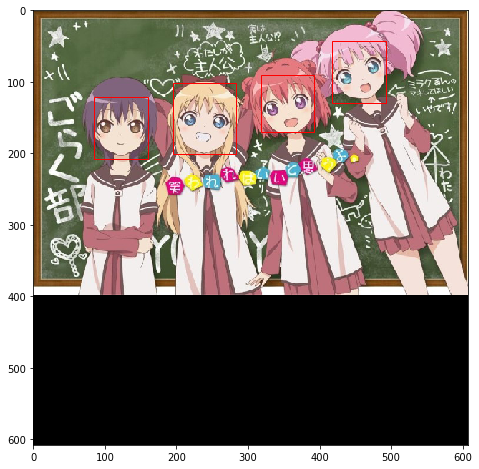
\includegraphics[width=7cm]{image/yolo_example.png}
\end{figure}
\begin{figure}[h]
  \centering
  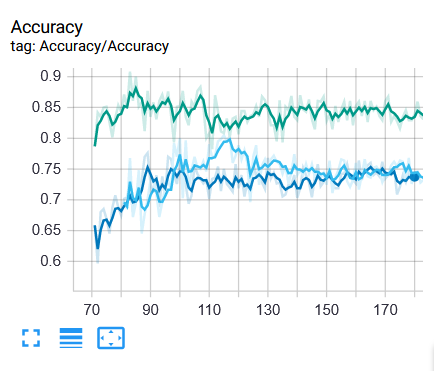
\includegraphics[width=7cm]{image/yolo_accuracy.png}
\end{figure}

The model showed 86\% of accuracy throughout the test dataset given. Focusing on
the precision than recall, consistent modification of hyper-parameters related
to the loss function was made. Unfortunately, the model tended to capture BBOXes
on the dataset without any faces, which led to significant false-positives. This
result was thought to be caused by the lack of datasets without faces in test or
validation datasets.

\subsubsection{Facial Expression Recognition}
\begin{figure}[h]
  \centering
  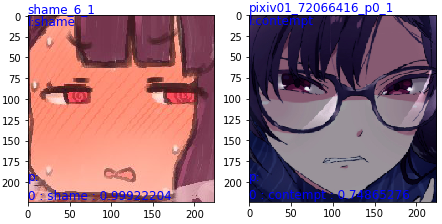
\includegraphics[width=7cm]{image/classifier_example.png}
\end{figure}

The model showed 43\% of accuracy for the case of Top 1, and 58\% for Top 2. At
first, accuracy was about 27\%. we tried supplying ~400 more datasets to the
training procedure and tuning hyperparameters led to 16\% accuracy increase. By
generating more training data, further accuracy escalation could be expected.

\subsubsection{Whole Applications of Models}
For each image inputs, we run YOLO with GMS to get BBOX for the face. For each
BBOX, we crop and resize each region to run classifier, just like general
2-staged object detectors.

\begin{figure}[h]
  \centering
  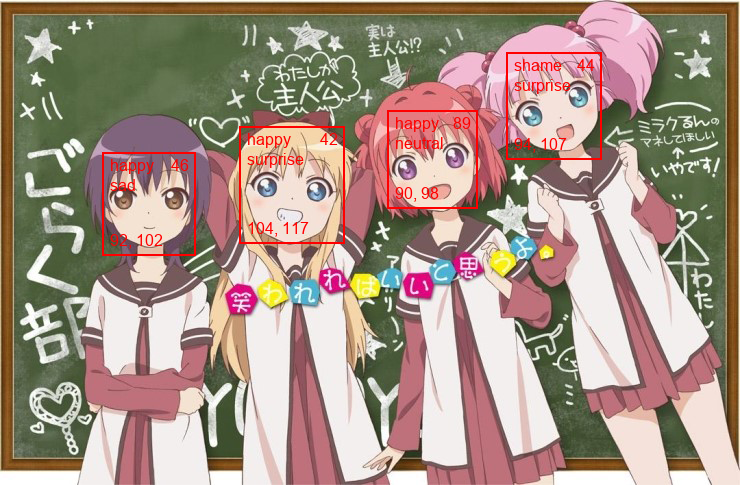
\includegraphics[width=7cm]{image/yolo_class_example.png}
\end{figure}

\section{State-of-the-Art}
Recent field of object detection has evolved to use multiple classifiers at a
time in a two-staged detectors - referred to as Cascade
R-CNN\cite{DBLP:journals/corr/abs-1906-09756}. Though YOLO is not a
State-of-the-Art technology, its fast training and detection speed made this
project to adapt it as first-staged object detection model. Also, making mask
data is a hard and laboring job, thus it was better to use simple and fast
framework for this project.

Facial Expression Classification has been a quite highlighted topic in deep
learning communities - it has also become far saturated topic. This project
adapted relatively shallow model among all presented models - otherwise the
machine could not train it properly.

\section{Challenges and Resolutions}
\subsection{Biased Dataset Problem}
The first problem this project faced was a bias in the dataset. Generally,
animation faces tend to have Happy or Neutral values for their expression
vectors. This feature led to the bias in the whole training set supplied to the
training process of the model.

To solve this problem, additional data were collected from varying sources other
than animations, to focus on removing the gap between the number of each feature
vectors. As a result, the test model was given ~120 datasets for each of the
vector elements.

\subsection{Subjective Dataset Labeling Problem}
In the dataset labelling process, there was a high chance of inappropriately
labelling expression vectors due to subjective labelling. Such dataset could
lead to an inaccurate or biased model.

For this problem, data was labelled to a certain expression only if two or more
team members agreed on the labelling result. This way, we tried to minimize the
subjectiveness in labelling procedure as possible.

\subsection{YOLO with NMS}
With a height and width of S=19 and anchor box count of 3, YOLO uses (anchor box
count * 21 * S * S) boxes, a total of 22743. For this heavy number of BBOXes,
NMS did not properly recognize faces, since there were too many BBOX around the
target.

Therefore, this project suggested a different approach, using a modified version
of NMS. Originally, in NMS, if IOU is larger than the pre-defined threshold, it
discards such BBOXes with smaller confidence. But intuitively, it is better to
hold such BBOX than just to discard it, for discarded boxes could also carry an
expected value on detecting objects. We have named this alternative approach as
Group Merge Suppression (GMS).

\lstinputlisting [style=custompy]{src/postprocess-algo.py}

To check whether GMS works better in practice than NMS, some data from the
test/validation set were given to each algorithm. By counting the result showing
higher IOU with the original BBOX, 68\% of result showed GMS performs better
than NMS.

\begin{figure}[h]
  \centering
  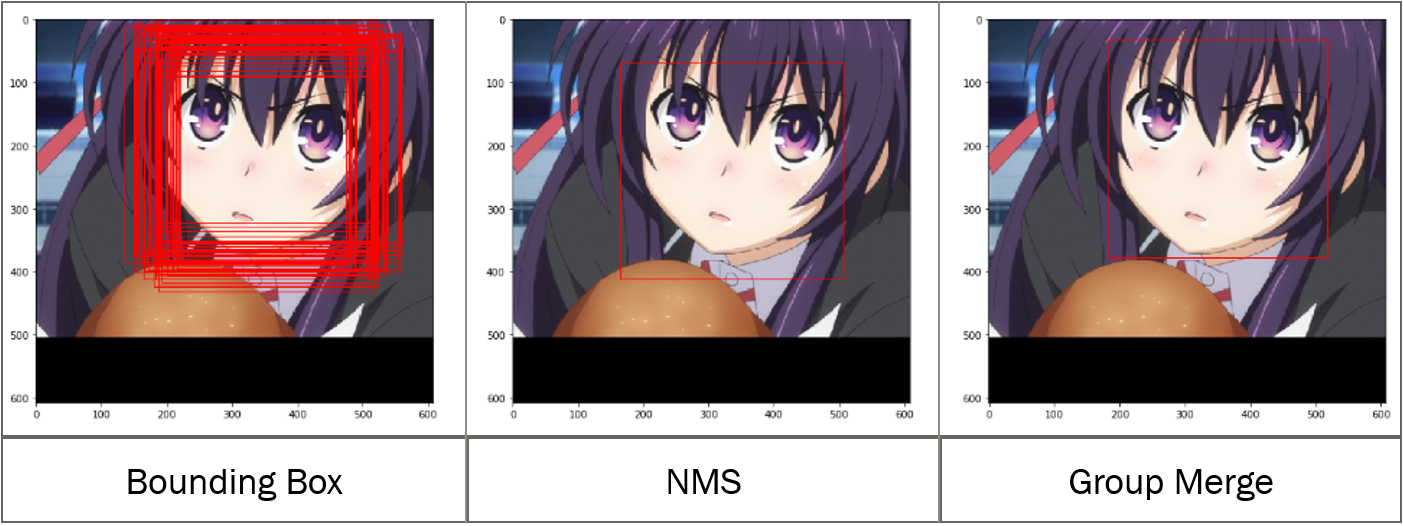
\includegraphics[width=7cm]{image/GMSvsNMS.png}
\end{figure}

\section{Future Direction}
\subsection{Segmentation}
The major problem during this project was the time required for manually
labelling data for model training. At first, segmentation was far complex: eyes,
hair, faces should have been marked with BBOX, individually.

The solution to this problem was to reduce the number of segmentation for a
dataset. In the latter process of labelling, BBOXes with face are forced to be
collected. This way, manual labelling time could be significantly reduced,
without any training problems regarding the dataset.

As a result, some data is labelled with more detailed segmentation. By using
this data and reinforcing them, more segmentation could be applied, as
Cascade R-CNN does in its network.

\subsection{Unification of Facial Expression Recognition within YOLO}
Originally, YOLO supports not only finding BBOXes of targets but also
classification based on data. Expression Classification is not an exception; the
classifier could be merged into YOLO to get the same result. Unfortunately, this
was not possible, due to the lack of hardware performance. If the hardware
holds, it could be a good approach, reducing the time and model complexity.

\subsection{Better BBOX Finding SSW}
For some case of the dataset, the model failed or poorly recognized to detect
the target. This is due to the lack of dataset and hardware performance. By
additionally supplying appropriate dataset to the model and going through more
trial-and-errors, better result and model could be expected.

\bibliography{final.bib}
\bibliographystyle{icml2019.bst}

\end{document}



